\documentclass{article}
\usepackage[utf8]{inputenc}
\usepackage{amsmath}
\usepackage{amsfonts}
\usepackage{hyperref}
\DeclareMathOperator*{\argmax}{arg\,max}
\DeclareMathOperator*{\argmin}{arg\,min}

\usepackage{graphicx}

\usepackage{array}
\newcolumntype{C}[1]{>{\centering\arraybackslash\hspace{0pt}}m{#1}}

\setlength{\parindent}{0cm}

\title{Udacity Navigation Project}
\author{Thomas Lecat}
\date{April 2021}

\begin{document}

    \maketitle

    \section{Environment}\label{sec:environment}

    The environment is described as Markov Decision Process $(S, A, R, p, \gamma)$ with unknown dynamics.
    The goal is to approximate the optimal policy $\pi^*$ that maximizes the upcoming cumulative reward in every state.

    This project uses value based methods, which seek to approximate the optimal $Q$ value $Q^*$, defined as:
    \[
    Q^*(s, a) = \max_{\pi} \mathbb{E}_{\pi} (\sum_{t} \gamma^t r_t | S_0=s, A_0=a),  \forall (a, s) \in A \times S
    \]

    Given $Q^*$, one can derive $\pi^*$ to solve the problem:
    $\pi^*(s) = \argmax_a Q^*(s, a), \forall s \in S$

    \section{Agent}\label{sec:agent}

    \subsection{DQN}\label{subsec:dqn}


    A vanilla \href{https://storage.googleapis.com/deepmind-media/dqn/DQNNaturePaper.pdf}{DQN} agent
    is implemented as the base solution.

    DQN approximates the $Q$ value by a neural network parameterized by $\theta$.
    Its loss function is defined as the mean squared TD error of the Bellman optimality equation:
    \[
    \mathcal{L}(\theta) = \mathbb{E}_{s, a, r, s'} \big[((r + \gamma \max_{a'} Q(s', a' | \theta^-)) - Q(s, a | \theta))^2\big]
    \]

    where $\theta^-$ are the parameters of a target network, slowly updated towards $\theta$ at every training step.
    This target network makes the TD target $r + \gamma \max_{a'} Q(s', a' | \theta^-)$ independent from the parameters $\theta$,
    which stabilizes the training.

    This loss is minimized by an Adam optimizer, a variant of the Stochastic Gradient Descent algorithm.
    At each step, the gradient is approximated from a minibatch of experiences ${(s, a, r, s', d)_i}$.
    To avoid a strong correlation between the steps of the minibatch, transitions are stored in a large replay buffer
    during rollouts and then sampled uniformly.

    \subsection{Double DQN}\label{subsec:double-dqn}

    The DQN agent is implemented in a modular way, to enable extension from recent papers to be added later.

    As a start, we implemented the improvements from the \href{https://arxiv.org/abs/1509.06461}{Double DQN} paper:
    Instead of using the target network to chose the next action and estimate its value in the target, use $Q_\theta$ to chose the action,
    and $Q_{\theta^-}$ to estimate its value.

    \section{Hyperparemeters}\label{sec:hyperparemeters}

    The network architecture is composed of 2 fully connected layers with 64 neurons each.
    The agent follows an $\epsilon$-greedy policy, with epsilon gradually decreasing from $1$ to $0.1$ over $30,000$ steps.

    The table below summarizes the main hyperparameters:

    \begin{tabular}{ |p{5cm} C{1cm}|p{3cm}|p{3cm}| }
        \hline
        \multicolumn{4}{|c|}{Hyperparameters} \\
        \hline
        \multicolumn{2}{|c|}{Parameter}   & Vanilla DQN & Double DQN                    \\
        \hline
        learning rate                     & $\alpha$    & \multicolumn{2}{|c|}{5e-04}   \\
        \hline
        discount factor                   & $\gamma$    & \multicolumn{2}{|c|}{0.99}    \\
        \hline
        target network update coefficient & $\tau$      & \multicolumn{2}{|c|}{0.001}   \\
        \hline
        buffer size                       &             & \multicolumn{2}{|c|}{100,000} \\
        \hline
        batch size                        &             & \multicolumn{2}{|c|}{64}      \\
        \hline
    \end{tabular}

    \section{Results}\label{sec:results}

    Both vanilla DQN and double DQN have been trained with 3 seeds.
    The reward curves are averaged over seeds and plotted below:

    \begin{figure}
        \centering
        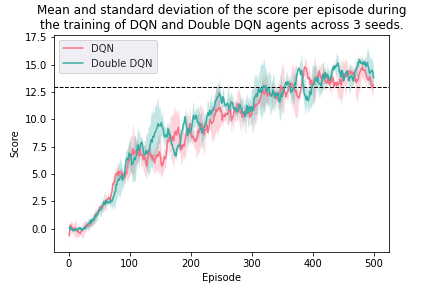
\includegraphics[scale=0.5]{results/reward_per_episode.png}\label{fig:figure}
    \end{figure}

    The addition of the double DQN strategy doesn't improve the results much and both
    agents manage to solve the environment in less than 400 episodes.

    \section{Next steps}\label{sec:next-steps}

    The next steps for the project consist in implemented other DQN extensions such as
    \href{https://arxiv.org/abs/1511.06581}{Dueling DQN} and
    \href{https://arxiv.org/abs/1511.05952}{Prioritized Experience Replay}.
    Hyperparemeters could also be further tuned using strategies such as
    \href{https://github.com/hyperopt/hyperopt}{HyperOpt} or
    \href{https://deepmind.com/blog/article/population-based-training-neural-networks}{Population Based Training}.

\end{document}
